\documentclass[conference]{IEEEtran}
\IEEEoverridecommandlockouts
% The preceding line is only needed to identify funding in the first footnote. If that is unneeded, please comment it out.
\usepackage{cite}
\usepackage{amsmath,amssymb,amsfonts}
% \usepackage{algorithmic} % unused template boilerplate
\usepackage{graphicx}
\usepackage{array}
\usepackage{float}
\usepackage{stfloats}
\usepackage{tikz}
% IEEEtran ends a run-in \paragraph head with a colon; use a period instead.
\makeatletter\renewcommand{\@IEEEsectpunct}{.\ }\makeatother
\usepackage{textcomp}
\usepackage{xcolor}
\usepackage[dvipsnames]{xcolor}
\usepackage{svg}
\def\BibTeX{{\rm B\kern-.05em{\sc i\kern-.025em b}\kern-.08em
    T\kern-.1667em\lower.7ex\hbox{E}\kern-.125emX}}
\usepackage{xcolor}

% Define color-coded author note commands.
% Set \shownotesfalse for the submission build to hide every note.
\newif\ifshownotes\shownotestrue
\newcommand{\SP}[1]{\ifshownotes{\color{blue}[SP: #1]}\fi}
\newcommand{\Sh}[1]{\ifshownotes{\color{red}{[Sh: #1]}}\fi}
\newcommand{\EK}[1]{\ifshownotes{\color{teal}{[EK: #1]}}\fi}
\newcommand{\QD}[1]{\ifshownotes{\color{ForestGreen}{[QD: #1]}}\fi}
\newcommand{\JW}[1]{\ifshownotes{\color{pink}{[JW: #1]}}\fi}
\newcommand{\todo}[1]{\ifshownotes{\color{yellow}{[TODO: #1]}}\fi}
\begin{document}

\title{What the Compiler Leaks: Attributing and Verifying Side Channels in Compiled ML Models\\
%{\footnotesize \textsuperscript{*}Note: Sub-titles are not captured in Xplore and should not be used}
%\thanks{Identify applicable funding agency here. If none, delete this.}
}
\author{anon for review}
%\author{\IEEEauthorblockN{1\textsuperscript{st} Given Name Surname}
%\IEEEauthorblockA{\textit{dept. name of organization (of Aff.)} \\
%\textit{name of organization (of Aff.)}\\
%City, Country \\
%email address or ORCID}
%\and
%\IEEEauthorblockN{2\textsuperscript{nd}FOO BAR}
%\IEEEauthorblockA{\textit{dept. name of organization (of Aff.)} \\
%\textit{name of organization (of Aff.)}\\
%City, Country \\
%email@address}
%\and ... 

%}

\maketitle

\begin{abstract}
Compilers are part of the confidentiality
boundary of machine learning systems, yet existing analyses
rarely distinguish information leakage originating in the source
program from leakage introduced or removed during compilation. A canonical example is constant-time cryptographic code:
libraries carefully preserve this property, yet aggressive compiler
optimizations can silently break it, introducing side channels.
Attackers can use these side channels to even leak confidential
weights of ML models. 
We then extend MLIR verification tools with SMT-based reasoning
and self-composition, so that each compilation step is checked
for computation the same result without new leakages. In the
Polygeist compiler, six of its eight compilation steps can be
checked this way on bounded inputs, and each check correctly
rejects a deliberately broken version of its step. These checks already
cover 8.2\% of the operations used in the Polygeist test suite.
\end{abstract}

\begin{IEEEkeywords}
side channels, constant-time, compilers, MLIR, translation validation, machine learning security
\end{IEEEkeywords}

%% prev version is https://pad.riseup.net/p/Mmc8qAM4NcZ7yr89sgPv 

\section{Introduction}
\label{sec:intro}

A deployed machine learning model never runs as it was written.
A compiler stack, such as PyTorch Inductor or an MLIR pipeline
followed by an LLVM backend, rewrites it into the code that actually
executes. What that code reveals through its branches, memory
addresses and timing is what an attacker observes. Such side channels
suffice to recover a model's architecture and even its
weights~\cite{batina2019csinn,yan2020cachetelepathy,hu2020deepsniffer},
so the compiler sits inside the model's confidentiality
boundary~\cite{chen2026compilerbackdoor,simon2018whatyouc}.

Cryptography has known this for a long time. Libraries written to run
in constant time are broken by compiler
optimizations~\cite{simon2018whatyouc,daniel2020binsecrel,kyberslash2024}.
Tools exist that detect the resulting
violations~\cite{almeida2016ctverif,daniel2020binsecrel},
and compilers exist that provably preserve the
property~\cite{barthe2020ctcompiler}.
That work targets hand-written cryptographic kernels and fixed C
compiler chains. Deep learning compilers are multi-level and
extensible, and they have neither. Validators for MLIR and LLVM check
that a transformation preserves computed
values~\cite{fcvd2025,lopes2021alive2,wang2024mlirtv},
not that it preserves secrecy. No existing analysis says, for an ML
workload, whether an observed leak was written in the source or put
there by the compiler.

The question matters more for a model than for a cipher.
Constant-time discipline assumes an ephemeral secret: a session key is
discarded before a channel yielding a fraction of a bit per run has
revealed anything. Model weights are frozen, and every forward pass
re-exposes the same secret, so an attacker with ordinary query access
averages a weak channel until it is clean. Inputs are the opposite
case. A token id is seen once, but an embedding lookup at a secret
index gives it away in a single cache observation. Both the weak
channels cryptographers dismiss and address-shaped channels therefore
matter, and for each we need to know what compilation does to it.

We call a \emph{channel} any observable of an execution that differs
between two runs with the same public inputs and different secrets.
The observables are which branches are taken, which addresses are
accessed, how long a variable-latency instruction runs, and how much
memory is allocated. We address channels from two sides. To
\emph{measure}, we build one kernel through several lowering pipelines
and optimization levels and run each binary on two classes of secret
input under Valgrind. Instruction, branch and write counts show that
the runs differ. Memcheck, used as a taint tracker~\cite{langley2010ctgrind},
shows which operand carried the secret to a branch or an address.
Comparing builds labels each channel as absent, present in both,
compiler-introduced or compiler-removed. Measurement speaks only about
the binaries we built. To \emph{verify}, we therefore write each
lowering step as a pair of source and target templates, with the
surrounding code left as uninterpreted holes, and discharge two SMT
queries on top of FCVD~\cite{fcvd2025}. The first requires the
target to compute the same results as the source. The second, built by
self-composition~\cite{barthe2004selfcomposition},
requires that any two runs the source cannot tell apart remain
indistinguishable in the target. A step is safe only if both hold.

Three findings run through the results. First, compilation is not
monotonically bad for confidentiality. A branchless
\texttt{arith.select} on a secret mask is still a \texttt{select} in
LLVM IR. The backend turns it into a conditional jump on the secret at
\texttt{-O0} and into a branch-free vector blend at \texttt{-O2}, so
the same toolchain introduces the channel and removes it. Second, a
leak can be invisible to every instrument that counts work. MLIR's
sparsifier moves a secret coordinate into a store address. Both secret
classes execute identical numbers of instructions, branches and
writes, and they differ only in where the writes land. Only taint
tracking reports it. Third, neither verification property subsumes
the other. A rewrite that forwards a stale value adds no observation
and passes the leakage check while computing the wrong result. A
rewrite that branches on a secret computes the right result and passes
any equivalence check. Either check alone certifies a real bug as
safe.

This paper makes the following contributions.
\begin{enumerate}
  \item A differential measurement method and kernel corpus that
    attribute each channel to the source or to the compiler across six
    MLIR pipelines at \texttt{-O0}, and three LLVM optimization levels on
    the baseline pipeline. Taint is the
    primary evidence. Count differences are admitted only past guards
    against a memory-layout confound that otherwise produces false
    positives. Applied to PyTorch Inductor, the same method shows that
    constant folding under weight freezing writes a weight-derived
    quantization scale into the generated code, a leak that is
    readable without running the model.
  \item Two-property translation validation for MLIR lowerings: a
    leakage model with four obligations (control, address, latency,
    resource), templates whose holes leave the surrounding code symbolic
    and whose shapes are swept over a declared range, and three-valued
    verdicts in which an unknown is never counted as secure.
  \item An application to Polygeist's eight-step C-to-LLVM
    pipeline~\cite{moses2021polygeist}.
    Six steps carry a bounded, two-property check of a rewrite
    transcribed from the pass source, each paired with a faulty control
    that the check rejects. Two steps are blocked by our sequential
    memory model and reported as such. A coverage measurement by
    translation, not by operation name, shows how far this is from the
    compiler's own test programs: 8.2\% of their operation mentions
    translate today.
\end{enumerate}

Section~\ref{sec:threat} fixes the threat model every later verdict is
stated against: which observer is watching, which asset is at stake,
and whether the leak occurs during a run or persists in what the
compiler leaves behind. Section~\ref{sec:evaluation} works through small
examples that fix the boundaries of each method.
Section~\ref{sec:measure} presents the measurement method and results,
and Section~\ref{sec:verify} the verification method and its
application to Polygeist. Section~\ref{sec:related-work} discusses related
work, Section~\ref{sec:discussion} limitations, and
Section~\ref{sec:conclusion} concludes.

\section{Threat Model}
\label{sec:threat}
% tikz is loaded in the preamble of the main file. Packages must not sit in the body.
% Source of truth, threat-models.agents.md and formal_verif.threat-model.agents.md.
% Limitations belong to the Discussion, not here.
A confidentiality claim about a compiler is empty until three questions have been answered.
Who is watching, what is that observer after, and at which stage of the toolchain the leak appears.
The first answer follows the usual practice of ranking observers by
how directly they reach secret state rather than by how powerful they
are assumed to be: side-channel taxonomies place attackers by
proximity~\cite{spreitzer2018classification}, and constant-time
leakage models nest so that a proof against a stronger observation
carries over to weaker ones~\cite{molnar2005pcmodel,almeida2016ctverif}.
We arrange eight such observers in rings so that every verdict in this
paper can be pinned to one.
The second question is where deep learning parts company with cryptography, because the assets of a model deployment are exposed on a schedule no cipher is ever exposed on, and it is that schedule, not the width of the channel, which decides what counts as a leak worth fixing.
The third question allows an observed channel to be charged to the source or to the compiler, which is the distinction our four-valued verdicts rest on.
Two of our findings are caused unambiguously by the compiler, neither of them is observed while a program runs, and so persistence is named here as a leak class of its own, which may be found only after execution ends.
\subsection{Observers}
\label{sec:threat:rings}
An observer is fixed by two things, the channel it reads, functional or timing or microarchitectural or power, and its position with respect to the secret.
For position we use eight rings, ordered so that every observer that infers sits outside every observer that reads.
Table~\ref{tab:rings} lists them and Fig.~\ref{fig:onion} draws the same ordering as nested reach. An observer placed on an outer ring holds strictly less than one placed inside it. The dashed circle marks where inference stops being necessary rather than where it stops being possible, since an observer inward of it already reads process memory.
\begin{figure}[t]
\centering
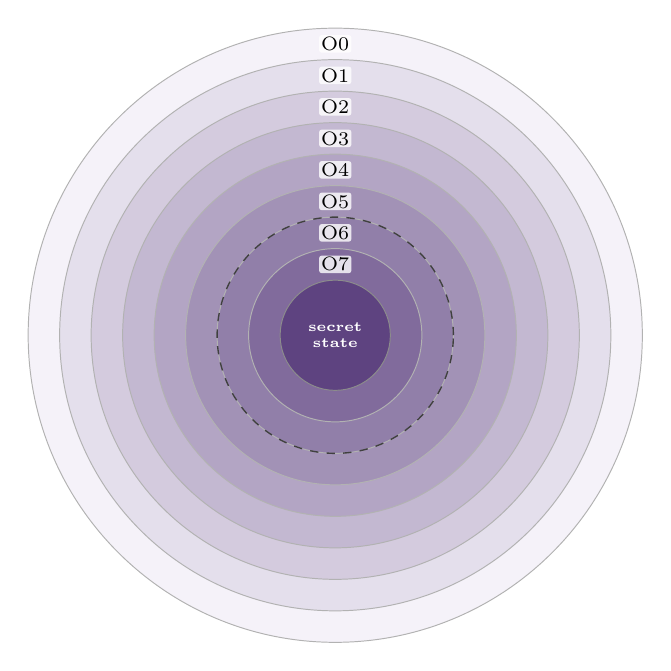
\begin{tikzpicture}[font=\scriptsize,line width=0.35pt]
  \definecolor{ringout}{HTML}{F5F2F9}
  \definecolor{ringin}{HTML}{5E4380}
  \foreach \i in {0,...,7} {
    \pgfmathsetmacro{\r}{3.90-\i*0.40}
    \pgfmathsetmacro{\mix}{11*\i}
    \fill[ringin!\mix!ringout,draw=black!30] (0,0) circle (\r);
  }
  \fill[ringin,draw=black!45] (0,0) circle (0.70);
  \foreach \i/\lab in {0/O0,1/O1,2/O2,3/O3,4/O4,5/O5,6/O6,7/O7} {
    \pgfmathsetmacro{\y}{3.90-\i*0.40-0.20}
    \node[inner sep=0.8pt,fill=white,fill opacity=0.80,text opacity=1,
          rounded corners=1pt] at (0,\y) {\lab};
  }
  \node[white,align=center,font=\tiny\bfseries] at (0,0) {secret\\state};
  \draw[dashed,black!75,line width=0.5pt] (0,0) circle (1.50);
\end{tikzpicture}
\caption{An observer model}
\label{fig:onion}
\end{figure}
\begin{table}[t]
\caption{Observer rings, ordered by directness of reach.}
\label{tab:rings}
\centering
\small
\begin{tabular}{@{}l@{\hspace{1em}}p{0.78\columnwidth}@{}}
\hline
ring & what the observer holds \\
\hline
O0 & outputs, errors, response length \\
O1 & latency measured end to end, repeated query statistics \\
O2 & branches, address classes, latency classes \\
O3 & cache sets and lines, pages, predictors, contention \\
O4 & power, EM, acoustic, thermal, frequency \\
O5 & the powers of a host minus whatever an enclave declares unreachable \\
O6 & process memory, registers, logs, files, core dumps \\
O7 & buses, internal memories, chip probes \\
\hline
\end{tabular}
\end{table}

A property proved at O2 carries outward to O1 and to O0.
A property that fails at O3 fails at O4 and at O5 as well, since the outer observer holds everything the inner one holds and more.
Inward of O6 the question dissolves rather than staying open, because an observer that already reads process memory has nothing left to infer.
Every verdict below is stated against a ring, and the two halves of the paper meet at O2, where the measurements bound the channel from below and the proofs discharge it from above.
A ring says how much an observer can see.
It does not say what a single operation gives away, and that finer vocabulary is what the leakage model of our checker supplies, sorting observations into the control, address, latency and resource obligations of \S\ref{sec:verify}.
The two are one axis read at two granularities.
The ring is the unit in which a verdict is stated and an attack is priced, the obligation kind is the unit in which a verdict is discharged and a channel is named, and a control obligation or an address obligation is nothing other than an O2 observation refined into the operand that produces it.
\subsection{Which asset, and therefore whether repetition helps}
\label{sec:threat:asset}
O2 is precisely the ring that classical constant-time discipline addresses, since the discipline demands that the sequence of branches and the sequence of memory addresses be independent of the secret, and it is that discipline our proofs discharge.
What the discipline assumes without saying so is that the secret is ephemeral.
A session key is used a bounded number of times and then discarded, so a channel yielding a small fraction of a bit per execution recovers nothing before the secret has gone.
A model deployment breaks the assumption, and it breaks it in opposite directions for the two assets that matter.
Weights are frozen, and every forward pass re-exposes the same secret.
A weak and noisy channel together with ordinary API access is therefore sufficient, because the attacker averages until the channel is clean.
Time works for him rather than against him, and a leak a cryptographer would dismiss as unexploitable is decisive here.
Recovery of architecture and of weights from cache~\cite{yan2020cachetelepathy}, from architectural observation~\cite{hu2020deepsniffer} and from electromagnetic observation~\cite{batina2019csinn} all run on this budget.
Inputs are the mirror image.
A token id is seen once, repetition buys nothing, and so the channel has to resolve the secret inside a single execution, which happens exactly when the leak is address shaped and the secret is small.
An embedding row gather at a secret token id is the clean case.
A single cache line observation narrows a vocabulary of thousands of entries substantially, in one query, with no averaging at all.
The two assets therefore do not merely differ in value, they make different leaks matter.
Variable latency arithmetic on a weight is a slow grind that repetition eventually wins.
A gather on a token id is immediate.
A third asset sits between the two and behaves like neither.
The architecture itself, together with tensor shapes, extents and sparsity or pruning patterns, is static and coarse, and it leaks through control structure rather than through values, which makes it invisible to any instrument that follows value flow and plainly visible in the address channel of a sparsity aware lowering.
It is also the asset the compiler reaches first, and the case studies below are where that shows: a secret extent used as a loop bound stays control-flow distinguishable at every pipeline and optimization level we tested, and sparsification moves a secret coordinate into a store address while leaving every aggregate count identical.
\subsection{Persistence, the attacker who arrives after the run}
\label{sec:threat:persistence}
Rings O0 to O5 all describe an observer of a running program, and each
of them needs co-residency or query access. An observer of the
persistent output of the compiler needs neither. The artifact exists
before the program has ever been run, it survives every run, and
reading it costs one call to \texttt{open}. Constant folding under
weight freezing writes a scale derived from $\max|w|$ into the generated
code as a literal, so whoever reads the artifact recovers that scale
exactly, without running the kernel and without timing anything. This
is not an accident of one optimization but the general shape of
quantized deployment: narrow numeric formats cannot represent a
tensor's dynamic range, so every quantized tensor ships a scale computed
from its largest magnitude, per tensor for int8 and
FP8~\cite{fp8formats}, per block of sixteen elements for
NVFP4~\cite{nvfp4} and thirty-two for MX~\cite{ocpmx}. Each scale is a function of the largest
magnitude in its scope, the maximum itself for per-tensor formats, an
FP8 value derived from it for NVFP4 and its exponent for MX, stored apart from the weight data and carried
through the pipeline as metadata. The folded literal we measure in
\S\ref{sec:production} is one instance of a statistic that every such
deployment writes into its artifact by design. Ahead-of-time
compilation goes further and bakes raw weight bytes into a shared
object that sits under a directory chain traversable by others and
outlives the compiling process.
 
Shapes leak by a parallel route. A compiler that specializes a tensor
dimension to a constant fixes that size into the generated code, so a
size derived from a protected extent becomes a secret written into the
artifact: the dynshape kernel of \S\ref{sec:evaluation:structure}, one level up. A
compiler that specializes must also re-check its assumption on every
call, a runtime comparison on the architecture
asset~\cite{pytorch2}. The two routes are not arbitrary. A compiler
reasons about a program on tensors that carry shapes but no data, so
anything it can derive from shape alone can be fixed into the artifact,
while anything that depends on the values reaches it only through a
deliberate exception. The artifact holds a program's shapes by default
and its weights only when the compiler is told to treat them as
constants.
 
None of these leaks is functional, since nothing was returned, nor
timing, since nothing was timed. No shared hardware state is involved,
so none is microarchitectural, and nothing was measured through power.
The closest fit in the ring vocabulary is O6, which does list files,
but O6 is moot by the argument above, and an attacker who can open a
file under a different UID holds no process memory whatsoever. That
attacker is strictly weaker than O6 and unlike anything in O0 to O5.
The standard grid conflates two entirely different observers, and our
clearest compiler-introduced results fall into the gap between them. We
therefore add persistence as a leak class, defined by the single
property that separates it from the other four: the attacker arrives
later, and reads rather than watches. It has two subcases. Build-time
residue is the artifact. Runtime residue is memory, swap, core dumps,
spilled registers, a reused connection pool, or GPU scratch left behind
for the next tenant.
 
Runtime residue is also a compiler problem, and for a structural
reason. A program that clears a secret before releasing its buffer
writes to memory that nothing reads again; to the abstract machine the
language defines, that store is dead, and removing it is a correct
optimization. Dead-store elimination does exactly this to scrubbing
code, a case D'Silva, Payer and Song place at the centre of the gap
between compiler correctness and security~\cite{dsilva2015gap}.
Yodaiken makes the general point from the side of systems programming:
the language standard, not the programmer's intent, decides what a
compiler may remove, and what systems code relies on the standard often
does not guarantee~\cite{yodaiken2021iso}. MLIR is no different, since
a deallocation promises nothing about the contents it releases. This is
why correctness of a lowering, the property the verifiers of
\S\ref{sec:verify} inherit, cannot rule out a persistence leak.
 
Naming the class rather than filing it under the nearest ring is the
same discipline this paper applies to what its methods cannot state: a
gap that is reported is a different object from a gap that has been
quietly counted as secure.
\subsection{Where this bites}
\label{sec:threat:deployments}
Four deployments fix different combinations of asset, observer and leak class.
The first is confidential inference inside a TEE.
The weights are the asset, the observer is O5 and close to an oracle, since controlled channel attacks resolve at the granularity of a 4 KB page~\cite{xu2015controlled} and single stepping resolves per instruction~\cite{vanbulck2017sgxstep}, and weight confidentiality is the guarantee the deployment advertises, so a secret dependent gather is a direct break and not a hypothetical one.
The second is multi-tenant serving, where both assets are present with opposite economics, where the observers are O3 and a persistence reader, and where one asymmetry decides everything.
The platform compiles, so the platform picks the optimization flags, the cache directory and the umask, while the tenant owns the weights and picks none of the three.
The third is on device and edge deployment.
Here the adversary owns the hardware, holds O3, O4, O6 and O7 and holds the artifact as well, and the honest aim is to raise cost rather than to close the channel.
The fourth is compiling for obliviousness.
The job of the compiler is then to emit data oblivious code, a leak is not an accident of optimization but a correctness bug inside a security mechanism, and this is why pass by pass verdicts are directly actionable.
When one pass closes an address channel while another opens a control channel, only the whole pipeline is safe, and whoever runs the first pass alone is not.

% Binary and symbolic results in III-A--III-C: 2026-09-14 artifact run.
% Source revision: 6e61076262dd06a711778489a0dea55af890ff40.
% Evidence: aisec-invariants-mlir/docs/research/satml-section3-results-20260914.agents.md.
% III-E incorporates the 2026-09-14 Overleaf contribution; its static comparison
% and regression claims were not rerun in the artifact batch above.
% This file uses only packages already present in the paper.
\section{Case Studies and Analysis Boundaries}
\label{sec:evaluation}

These cases show how lowering changes observable behaviour, why correctness and leakage require separate checks, and what each analysis can establish.

We compare each kernel on two chosen secret inputs while keeping its public inputs fixed.
Callgrind records the total numbers of executed instructions (Ir), conditional branches (Bc), and memory write references (Dw) around the kernel call, excluding input loading and program setup.
These execution counts do not measure elapsed time.
In separate runs, Memcheck tracks the secret input and reports when it influences a conditional jump or move (\texttt{cf}) or a memory address (\texttt{addr}).
Thus counts and secret-dependent conditions or addresses are separate observations.
Each count comparison uses five paired runs under the measurement procedure described in Section~IV.

We use MLIR and Clang 18.1.3, Valgrind 3.22.0, and an AMD Ryzen AI 9 HX 370 running Linux x86-64.
Core kernels follow the baseline \texttt{linalg}--\texttt{scf}--\texttt{cf}--LLVM lowering (P0), compiled with \texttt{-mavx2 -mno-avx512f} at \texttt{-O0}, \texttt{-O2}, and \texttt{-O3}.

\subsection{Select and Backend Lowering}
\label{sec:evaluation:select}

The \texttt{mask\_select} kernel selects between two public arrays using a secret byte mask.
It loads both candidate values and applies \texttt{arith.select} in a fixed-size traversal, without branching on the mask.
The lowered LLVM IR retains \texttt{select}; the secret-dependent branch appears during backend compilation at \texttt{-O0} (Figure~\ref{fig:select-lowering}).

\begin{figure}[!ht]
\centering
\begin{minipage}{0.97\columnwidth}
\footnotesize
\setlength{\topsep}{2pt}
\textbf{Source MLIR and lowered LLVM IR}
\begin{verbatim}
%c = arith.cmpi ne, %m, %zero : i8
%s = arith.select %c, %av, %bv : f32
...
%39 = select i1 %38, float %34, float %37
\end{verbatim}
\textbf{O0: the mask controls a jump}
\begin{verbatim}
3550: cmp $0x0,%al
3558: jne 356a <mask_select+0x9a>
\end{verbatim}
\textbf{O2/O3: the vector path uses a blend}
\begin{verbatim}
2df2: vpcmpeqd %ymm0,%ymm1,%ymm1
2df6: vblendvps %ymm1,(%rdx,%rax,4),
                %ymm5,%ymm1
\end{verbatim}
\end{minipage}
\caption{Measured select lowering. Surrounding loads and public loop/alias checks are omitted; the blend instruction is wrapped. LLVM IR retains selection until backend compilation.}
\label{fig:select-lowering}
\end{figure}
% Coauthor note kept from the Overleaf version:
% \EK{I believe we could remove code freely to save space - we have 13 pages already}

% Author question addressed by the measurement paragraph above:
% \SP{We should give some background on what is being measured and how}
At \texttt{-O0}, the all-one mask executes 8,192 fewer instructions and 4,096 fewer write references than the all-zero mask.
Both executions encounter the same number of conditional branches, but Memcheck identifies a branch whose condition depends on the mask.
Equal branch counts therefore do not imply equal branch outcomes.

% Author question addressed by specifying the kernel call below:
% \SP{What is a marked region?}
The exercised vector path uses \texttt{vblendvps} at \texttt{-O2} and \texttt{-O3}.
Memcheck reports no secret-dependent conditional jump, conditional move, or memory address during the kernel call, and the two masks produce identical instruction, branch, and write-reference counts.
This result applies to the tested executions; it is not a proof of constant-time behaviour.

% \SP{what is a conditional reduction?}
Table~\ref{tab:section3-core} compares the select with a fixed computation, a branch on a secret sum, a load at a secret index, and a loop with a secret extent.
The \texttt{cond\_reduce} kernel sums its secret array, then branches on whether the sum is positive to write either 1 or 2.

\begin{table}[t]
\caption{P0 results for the chosen inputs. Memcheck reports \texttt{cf} or \texttt{addr}; count difference denotes a stable difference in Ir, Bc, or Dw. A dash means no finding or count difference detected, respectively.}
\label{tab:section3-core}
\centering
\footnotesize
\setlength{\tabcolsep}{3pt}
\begin{tabular}{@{}lcccccc@{}}
\hline
& \multicolumn{3}{c}{Memcheck finding} & \multicolumn{3}{c}{Count difference} \\
\cline{2-4}\cline{5-7}
Kernel & O0 & O2 & O3 & O0 & O2 & O3 \\
\hline
\texttt{matvec} & --- & --- & --- & --- & --- & --- \\
\texttt{cond\_reduce} & \texttt{cf} & --- & --- & Yes & --- & --- \\
\texttt{mask\_select} & \texttt{cf} & --- & --- & Yes & --- & --- \\
\texttt{idx\_gather} & \texttt{addr} & \texttt{addr} & \texttt{addr} & --- & --- & --- \\
\texttt{dynshape} & \texttt{cf} & \texttt{cf} & \texttt{cf} & Yes & Yes & Yes \\
\hline
\end{tabular}
\end{table}

\subsection{Shape and Sparsity}
\label{sec:evaluation:structure}

% \SP{stored-value counts?}
Confidential structure can influence execution even when tensor dimensions and the number of explicitly stored entries are fixed.
Our sparse example represents a vector of length 256 by eight stored values \(1,\ldots,8\), their coordinates, and a position array \([0,8]\).
% \SP{What is the difference between a position and a coordinate?}
% \SP{what is a public position array?}
% \SP{What is a coordinate, still unclear}
The positions are offsets into the stored-entry arrays: \([0,8]\) selects entries 0 through 7.
Each coordinate gives the index in the length-256 vector where its associated value belongs.
The vector length, values, and positions are public, meaning the observer may know them, and are identical in both inputs.
Only the coordinate array changes: the first input uses \([0,1,2,3,4,5,6,7]\), while the second uses \([3,29,61,97,130,168,201,240]\).

\paragraph{From representation to address}
The source first assembles values, positions, and coordinates into a compressed sparse tensor, then converts it to a dense tensor.
We apply MLIR's sparsifier with its runtime-library mode disabled, followed by LLVM conversion and a Clang \texttt{-O0} backend.
The code zeroes a fixed-size output, then iterates over the eight stored entries.
The public position array determines the loop bounds; each secret coordinate determines a store address (Figure~\ref{fig:sparse-address}).

\begin{figure}[!ht]
\centering
\begin{minipage}{0.97\columnwidth}
\footnotesize
\setlength{\topsep}{2pt}
\textbf{Dense materialization, summarized as pseudocode}
\begin{verbatim}
out[0:256] = 0
for i in pos[0]:pos[1]:     # public range
    c = crd[i]             # secret coordinate
    out[c] = vals[i]       # secret address
\end{verbatim}
\textbf{Generated address and store, with SSA names shortened}
\begin{verbatim}
%c = llvm.load %crd_ptr : !llvm.ptr -> i64
%p = llvm.getelementptr %out[%c]
     : (!llvm.ptr, i64) -> !llvm.ptr, f32
llvm.store %v, %p : f32, !llvm.ptr
\end{verbatim}
\textbf{Machine instruction reported by Memcheck}
\begin{verbatim}
1976: movss %xmm0,(%rcx,%rdx,4)
\end{verbatim}
\end{minipage}
\caption{The sparse-to-dense lowering uses a secret coordinate as a store index. The public number of iterations does not determine the sequence of addresses.}
\label{fig:sparse-address}
\end{figure}

\paragraph{Equal counts, different addresses}
The scatter loop performs eight stores for either coordinate pattern, but their destination addresses differ.
The sparse binary has equal instruction, branch, and write-reference counts in all five paired runs, while Memcheck reports a store address that depends on the secret coordinate.
The \texttt{idx\_gather} example shows the same distinction at all three optimisation levels.
Equal counts do not rule out secret-dependent addresses, though these experiments do not measure cache-line visibility or physical timing.

The separately authored dense reference visits all \(256\times8\) position-entry pairs and uses loop-derived load and store addresses.
No secret-dependent address is detected in that build, but its \texttt{-O0} binary contains a secret-dependent \texttt{je}, confirmed at the instruction identified by Memcheck.
Its execution counts also remain equal across the two coordinate inputs.
The comparison distinguishes their address channels; the reference already has a control channel.
As these are separate source programs without a complete output comparison, the experiment does not establish functional correctness of the sparse lowering.

\paragraph{Dynamic extent and bufferization}
The \texttt{dynshape} kernel makes the allocation size and loop bound depend on a secret extent \(k\).
% \SP{What is a backend level, do you mean opt level?}
For \(k=1\) versus \(k=4096\), Memcheck reports a secret-dependent condition at all three P0 optimisation levels.
The instruction difference falls from 73,872 at \texttt{-O0} to 5,117 at \texttt{-O2}/\texttt{-O3}; the write-reference difference falls from 20,493 to zero as the write-only buffer is eliminated.
This experiment starts from \texttt{memref} operations.
Attributing a channel to one-shot bufferization requires comparison with the corresponding tensor program lowered through that pass (P4).

\subsection{Two Distinct Verification Obligations}
\label{sec:evaluation:polygeist}

A transformation can compute the wrong result without adding leakage, or preserve the result while adding an observation.
We check four hand-transcribed Polygeist transformation specifications: two faithful examples and two deliberately modified versions.
The equivalence check compares returned values and modeled final memory under the checker's refinement relation.
The leakage-preservation check asks whether source-indistinguishable executions remain target-indistinguishable:
% \SP{What do these symbols mean?}
\[
  L_S(x)=L_S(x')\ \Longrightarrow\ L_T(x)=L_T(x').
\]
Here \(L_S\) and \(L_T\) are the source and target observation traces, and \(x,x'\) agree on public inputs.
The source may already leak; the target must not distinguish inputs the source's observations leave indistinguishable.
The two obligations are logically distinct but share the SMT encoding infrastructure.
Table~\ref{tab:gate-controls} uses the supported observation model with the \texttt{--unroll 8} truncation limit.
The faulty specifications are deliberate modifications, not discovered upstream compiler bugs.


Propagating an unchanged loop-carried value passes both checks.
The modified specification substitutes its initial value after it changes: the returned accumulator exposes the error, while the leakage check passes.
The faithful loop restructuring also passes both checks.
Moving its body before the first condition check fails leakage preservation but passes equivalence for this example's returned flag.
The flag is false within the modeled executions; this does not establish that arbitrary loop bodies can be moved safely.

Verification succeeds only when both checks pass; each rejected specification returned a counterexample.
All four results concern the model truncated with \texttt{--unroll 8}; the saved loop counterexample is sensitive to that truncation.
For CFG loops, the limit counts visits per block rather than restricting input bounds to eight completed iterations.
Unspecified computations, called holes, are symbolic functions shared between source and target, with effects and observations limited by the model.
The results cover these specifications, not production passes, unbounded loops, or downstream executables.

\subsection{Analysis Boundaries}
\label{sec:evaluation:boundaries}

Table~\ref{tab:analysis-boundaries} compares the methods' scopes: one IR stage, symbolic inputs under a truncated model, or an executable on chosen inputs.


The select has no secret branch in the inspected IR but has one in the \texttt{-O0} executable: the compilation stage matters.
Gather and sparse materialization use secret-dependent addresses despite equal counts: the observation matters.
No method supplies universal ground truth for the others.

Unsupported encodings, timeouts, and solver unknown responses yield \texttt{UNKNOWN}; none occurred in the four verification examples.
A bounded result is not automatically \texttt{UNKNOWN}.
IR analysis reports some unsupported operations, but missing dependency propagation rules can cause missed findings.
Without validated rule coverage, an IR result with no finding does not establish obliviousness.
The comparison in Section~\ref{sec:evaluation:static} concerns five kernels under the stated lowerings; agreement on that corpus does not establish complete rule coverage or general analyser accuracy.

\subsection{Static prediction against measured ground truth}
\label{sec:evaluation:static}
% Imported comparison: verify the exact static-analysis revision, commands,
% per-pipeline outputs, regression test, and runtime before submission.

Measurement (§IV) speaks about the binary that ran, at one configuration and for two input classes.
Symbolic verification speaks about inputs within its supported execution and observation model.
A third tier sits between them: a forward taint analysis over the MLIR as given, needing no flattening, solver or per-operation semantics, and reasoning about the IR rather than the downstream binary.
An all-inputs conclusion requires sound propagation rules for the supported IR.
This subsection defines it and asks whether its verdicts agree with what the binary did.

\paragraph{What the analysis is} A function argument marked secret taints its value, and taint propagates forward: any operation with a tainted operand taints all of its results, a store taints the buffer it writes, a yield taints both the parent operation's result and the loop argument it re-binds, and a branch's successor operands taint the block arguments they reach.
These edges run in both directions around a loop, so the taint sets are iterated to a fixpoint rather than computed in one pass.
A tainted value that reaches a loop bound, a load or store index, or a branch condition is a violation on the control or address obligation.
Unsupported calls, buffer aliases, and opaque regions must produce an unknown result when their effects cannot be modeled.
The analysis uses forward taint propagation, as does the verifier's prefilter, but operates directly on unflattened IR.
This lets it inspect some programs that the flattener refuses; it does not establish that the two implementations have identical coverage.
That propagation is standard taint over ordinary MLIR annotations, and we claim nothing for it (discussed in related work).
What we claim is the comparison.

\paragraph{The comparison} The five kernels of §IV were run through the analysis before and after the MLIR pipelines described in Section~IV, at the same lowerings the rig measured, and the static verdict was set beside the measured one at -O0.
Table~\ref{tab:static-analysis-results} gives the result.

The comparison distinguishes five verdicts: \emph{oblivious}, meaning no finding before or after lowering; \emph{authored-and-survives}, a violation before and after; \emph{lowering-introduced}; \emph{lowering-removed}; and \emph{unknown-after}.
An unknown result after lowering must not be counted as removal.
The reported static verdicts are the same for P0--P3 and P5; P4 applies to the tensor kernels.
In Table~\ref{tab:static-analysis-results}, ``Authored'' abbreviates authored-and-survives.
Agreement compares the presence of a control or address finding, not equality of every observation.
The binary column retains the reported control and address findings; \texttt{Dw} denotes a difference in write-reference counts, rather than an additional static obligation.
The one-write difference for \texttt{cond\_reduce} accompanies its control finding and is omitted from this summary.

\begin{table}[t]
% \EK{Oh my Godness, wha happened}
\caption{Reported static and binary verdicts at \texttt{-O0}.}
\label{tab:static-analysis-results}
\centering
\footnotesize
\setlength{\tabcolsep}{3pt}
\begin{tabular}{@{}lccc@{}}
\hline
Kernel & Binary & IR before/after & Agree \\
\hline
\texttt{matvec} & Oblivious & Oblivious & Yes \\
\texttt{cond\_reduce} & \texttt{cf} & Authored (\texttt{cf}) & Yes \\
\texttt{idx\_gather} & \texttt{addr} & Authored (\texttt{addr}) & Yes \\
\texttt{dynshape} & \texttt{cf}+\texttt{Dw} & Authored (\texttt{cf}) & Yes \\
\texttt{mask\_select} & \texttt{cf} & Oblivious & \textbf{No} \\
\hline
\end{tabular}
\end{table}

The reported verdicts agree on four of five kernels; the disagreement has a compilation-stage explanation.
At the MLIR level \texttt{mask\_select} has no secret-dependent branch or address; \texttt{arith.select} on the mask is exactly what the analysis models, and a finding-free result is consistent with that source structure.
The measured branch appears during LLVM backend compilation at \texttt{-O0} (Section~\ref{sec:evaluation:select}), after the inspected IR stage; at -O2, where the selector emits a blend, the measured result has no finding and the two tiers agree again --- with the static tier having seen neither the introduction nor the removal.
The comparison illustrates the compilation-stage limit described in Section~\ref{sec:evaluation:boundaries}.
Agreement on these kernels is not a general accuracy or soundness guarantee.

\paragraph{A false verdict caught by measurement} The comparison did work beyond confirming agreement.
An earlier form of the analysis lost taint across \texttt{--convert-scf-to-cf}: it tracked \texttt{scf} conditions but not the \texttt{cf.cond\_br} they lower to, so one standard lowering step later it went blind.
A before/after run then read that blindness as lowering-removed --- the compiler appeared to have fixed \texttt{cond\_reduce}, whose \texttt{-O0} binary is reported to retain a control finding across the measured pipelines.
The blindness, not the compiler, had removed the leak.
The reported fix propagates the missing edges and adds a regression kernel, but the lesson generalizes to any differential analysis: a verdict of removed is trustworthy only if the analysis can still see the program after the step, and one that cannot must answer unknown-after --- which must never be folded into removed.

\paragraph{What the tier is for} It covers two of the four obligations, models no aliasing, is intraprocedural, and stops at the MLIR boundary.
Within the supported IR it can propagate dependencies without translating each operation into SMT.
Its conclusions still depend on sound propagation and detection of unsupported constructs; the five-kernel comparison does not validate those properties for arbitrary programs.

\section{Measuring: Compiler-Introduced and Compiler-Removed Channels}
\label{sec:measure}

Given one kernel, one lowering pipeline and one optimisation level, is the binary's behaviour distinguishable across two classes of secret input, and if so, through which operand did the secret get there. The answer is a measurement, not a proof: it holds for the two classes it exercised, on the toolchain that built the binary, and it is reported with those coordinates attached. \S\ref{sec:evaluation:select} and \S\ref{sec:evaluation:structure} interpret the mechanisms; this section states the method and the full results.

\subsection{Methodology}

The rig builds one binary per cell, where a cell is one kernel lowered through one MLIR pipeline at one LLVM optimisation level, and runs it on two classes of secret input under two Valgrind tools. Callgrind, started and stopped around the kernel call, counts the instructions the simulated processor executed (Ir), the conditional branches it executed (Bc) and its write references (Dw). Memcheck, with the secret buffer marked undefined before the call, tracks definedness through every arithmetic and memory operation and reports where an undefined value reaches a conditional jump or move (the control channel, cf) or the address of a load or store (the address channel, addr). This is Langley's ctgrind construction~\cite{langley2010ctgrind}: Memcheck's definedness shadow bits serve as taint tags. Counts say that two runs did different amounts of work; taint says which operand carried the secret to an observation, and needs no magnitude.

Taint is primary and counts corroborate. A cell is distinguishable if Memcheck reports a channel or if a count differs between the classes, and a count difference on its own is admitted only past two guards, because the count channel has a confound that is not noise. Valgrind disables address-space randomisation, so memory layout is a deterministic function of a run's arguments and environment, and byte-identical secrets stored at file paths of different length execute counts that differ by several hundred instructions; repeating at one fixed path shows a spread of zero and hides this. Each class is therefore measured at five contexts of varying path length, paired by context, and a count difference is reported only if its median exceeds the largest spread either class shows across contexts (the floor) and the paired differences agree across contexts (stability). Layout manufactures false positives, never false zeros, so a count that fails a guard is uninterpretable rather than clean, and the layout-insensitive taint channel decides. Two consequences follow. Memcheck's control report covers a conditional move as well as a jump; a comparison alone does not necessarily trigger that diagnostic. Where this distinction matters, the verdict is taken on the address channel. And a leak whose only signature is the address touched is invisible to the counts and visible to Memcheck alone.

Secret classes are chosen, not sampled: each pair sits on opposite sides of the mechanism its kernel probes. Comparing two cells gives four outcomes. Relative to a baseline cell, a second cell is oblivious if neither leaks, leak-present if both do, introduced if only the second does and removed if only the baseline does; the baseline is a parameter of the run and is named in every report, and below it is the plain lowering at -O0 unless stated.

Every number below and in Section~\ref{sec:evaluation} comes from one run on one machine: an AMD Ryzen AI 9 HX 370 under Ubuntu 24.04 with mlir-opt 18.1.3, clang 18.1.3 with \texttt{-mavx2 -mno-avx512f} (Valgrind 3.22 does not decode AVX-512), Valgrind 3.22.0, glibc 2.39, kernels of 4096 elements and 256×256 matrices. The kernels that allocate pass through glibc's CPUID-dispatched routines, so their counts may differ on another processor.

\subsection{Kernels and the compiler axis}
Five kernels probe the obligations of \S\ref{sec:verify}, each with the two classes that bracket its mechanism: \texttt{matvec}, dense with fixed bounds, the negative control (zero weights against Gaussian); \texttt{cond\_reduce}, a branch on the secret sum (all zero against all one); \texttt{mask\_select}, a branchless \texttt{arith.select} on a secret mask (all false against all true); \texttt{idx\_gather}, a load at a secret index (index 0 against random); and \texttt{dynshape}, a secret extent used as allocation size and loop bound (1 against 4096). Tensor-typed variants \texttt{matvec\_t}, \texttt{mask\_select\_t} and \texttt{dynshape\_t} give one-shot bufferization real decisions to make; \texttt{scatter} under the sparsifier, against a hand-written dense reference, is described in Section~\ref{sec:evaluation:structure}.

The MLIR axis is six pipelines that differ only before a common tail into the LLVM dialect: the plain \texttt{linalg}→\texttt{scf}→\texttt{cf} path (P0), the affine path (P1), canonicalisation and CSE ahead of P0 (P2), affine super-vectorisation (P3), one-shot bufferization for the tensor kernels (P4) and generalisation of named ops (P5). The LLVM axis is -O0, -O2 and -O3. Section~\ref{sec:evaluation:boundaries} sets the IR-analysis verdict beside these P0 measurements; the analysis was not swept over the other pipelines.


\subsection{Results}

Table~\ref{tab:measured-cells} gives every cell of that run. The mechanisms behind its rows are the subject of \S\ref{sec:evaluation:select} (the select) and \S\ref{sec:evaluation:structure} (shape, bufferization, sparsity); two regularities of the table as a whole are stated here.


The MLIR axis moves magnitude; the LLVM axis moves verdicts. Across the five pipelines at -O0 no kernel's verdict or channel changes. Canonicalisation ahead of lowering (P2) makes \texttt{dynshape} execute 12,447 fewer instructions and perform 4,113 fewer write references in the class-B-minus-class-A difference, and reports the same channel with the same taint. Every verdict that changes in the table changes along the -O axis, and every channel that survives -O3 is one the program computes from its input: a runtime trip count or an address.

The count channel is blind to address leaks. \texttt{idx\_gather} and the sparsified \texttt{scatter} have identical counts in both classes at every cell and are reported by Memcheck alone. A rig that measured only work (instructions, branches, cycles) would return oblivious for both.

\subsection{A production compiler}\label{sec:production}

Before the MLIR corpus we ran the same methodology on PyTorch's Inductor backend (torch 2.13, CPU), eager against compiled, on an activation-function corpus of 512×512 inputs. In exp, with classes of 0.5 against 100.0 bracketing the overflow handling of a scalar exponential, the eager build executes 35,061,760 more instructions and 3,416,064 more branches for the large class and Memcheck traces the secret to a branch condition; the compiled build shows no difference and no report. The verdict is compiler-removed. The corpus was designed to probe a scalar libm expf in the eager kernel against a branchless vectorised polynomial in Inductor's generated code. \texttt{relu} is oblivious in both builds; \texttt{gelu}'s sweep did not complete; softmax's probe was degenerate (uniform rows) and is retained as a retired result.

Freezing with constant folding writes a scale derived from \texttt{max|w|} into the generated code as a literal. Running Memcheck on the compilation itself with the weight bytes marked undefined gives 184 reports at the float-formatting site of the code generator in the frozen configuration and none in the unfrozen control, and the emitted literal equals \texttt{max|w|/127} to float32 precision across seven perturbations of the weights. Nothing was executed and nothing was timed; this is the leak the threat model files under persistence. Autotuning is a clean negative: max-autotune selects the same GEMM kernel and emits generated code identical after normalisation across dense, sparse, low-rank, subnormal, small- and large-magnitude weight classes and across independent draws within a class, consistent with the tuner benchmarking on inputs of the right shape rather than on the weights.
\section{Verifying, Two-Property Translation Validation for a Real Pipeline}
\label{sec:verify}
% Source of truth, fcvd-verification-stages.agents.md for the protocol,
% fcvd-selfcomposition.agents.md, fcvd_ct/README.md, polygeist-verification journal.
% Numbers marked [measured] were printed by the tool on the dates given.
% REGENERATE from live data before submission. Limitations go to the Discussion.
Any measurement can only find the leakage channels that occur in the artifacts we happened to build, and so it speaks about a sample rather than about a compiler.
In place of that sample we offer a check on a lowering step that is discharged once for a specified family of instances of the step, with the surrounding code left symbolic, rather than for the handful of programs we happened to compile.
In what follows we describe the substrate we build on and what is missing from it before a security property can even be written down, then the protocol that turns such a property into a solver call, then the reason a single property is never enough, so that a step counts as specified only when two independent queries succeed, and finally a run of the whole construction on a production pipeline, the eight step lowering from C to LLVM inside Polygeist~\cite{moses2021polygeist}, which ends in a verdict for each step together with a coverage counter that recomputes on every run the arithmetic behind those verdicts.

An observation is what a single operation gives away to the observer of our leakage model.
An obligation is the proof duty attached to one kind of observation, namely the claim that the sequence of observations of that kind, taken together with the guards under which they occur, is identical in any two executions that agree on their public inputs.
We take exactly four obligations, and each of them is fed by a fixed set of operations.

The control obligation is fed by branches and loop bounds, which give away the condition they test and the trip count they produce.
The address obligation is fed by loads, stores, extracts and inserts, which give away the index operands they are addressed with, and after lowering to LLVM by address computations, loads and stores, which give away their offsets and pointers.
The latency obligation is fed by integer division and remainder, in the arithmetic and the LLVM dialects alike, which give away both of their operands, because the running time of these operations depends on them, and this is the very mechanism behind KyberSlash~\cite{kyberslash2024}.
The resource obligation is fed by allocation and deallocation, which give away the requested size and the freed block.
Nothing else is observed, so these four sentences are the entire leakage model, and every verdict we issue below names the obligation it discharges or refutes.

\subsection{From value semantics to a security property}
\label{sec:verify:fcvd}

The substrate is FCVD~ \cite{fcvd2025}, first class verification dialects for MLIR, which equips every MLIR operation with a formal SMT semantics.
A value in that semantics is a pair of a bitvector and a poison flag, memory is threaded through the program as an effect and lowered into SMT arrays, and undefined behaviour is carried by an explicit flag instead of being left implicit.
Lowering a function here means replacing each of its operations by the corresponding formula, after which a refinement query between two functions is one solver call and nothing beyond that.

FCVD can state that two programs compute the same values and cannot state that somebody watching one of them learns nothing about the secret, so a security property as it stands is simply not expressible in it.
The reason is structural: leakage freedom is not a property of a single execution but a 2-safety hyperproperty ~\cite{clarkson2010hyperproperties}, a statement relating two runs that share their public input, and no formula about one run can express it.
Two additions make it expressible, of which the first is the leakage model already given above, that is, a fixed declaration of which operations the attacker sees and which of their operands the sighting consists of, so that the act of watching becomes part of the semantics instead of remaining an informal side condition.
The second addition is self composition~\cite{barthe2004selfcomposition}, which is exactly the move that turns such a two-run hyperproperty into a property of one formula built from both runs.
Once both additions are in place, the constant time requirement collapses into a single satisfiability query, and the entire operation coverage of MLIR starts working for a security proof rather than for a correctness proof alone.

\subsection{The protocol}
\label{sec:verify:protocol}
\begin{figure}[t]
\centering
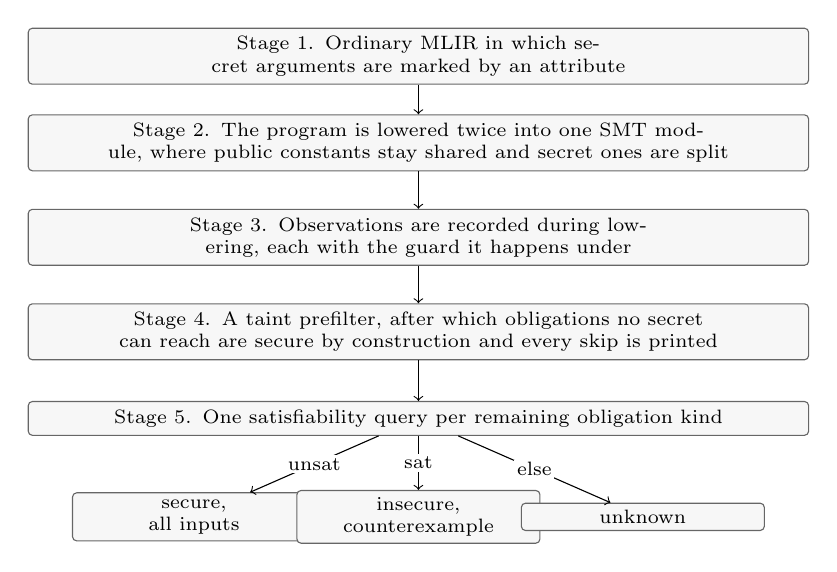
\begin{tikzpicture}[font=\scriptsize,line width=0.4pt,
  box/.style={draw=black!60,rounded corners=1.5pt,align=center,
              inner sep=3pt,text width=0.80\columnwidth,fill=black!3},
  vb/.style={draw=black!60,rounded corners=1.5pt,align=center,
             inner sep=2.5pt,text width=0.24\columnwidth,fill=black!3}]
  \node[box] (s1) at (0,0)
    {Stage 1. Ordinary MLIR in which secret arguments are marked by an
     attribute};
  \node[box] (s2) at (0,-1.10)
    {Stage 2. The program is lowered twice into one SMT module, where public
     constants stay shared and secret ones are split};
  \node[box] (s3) at (0,-2.30)
    {Stage 3. Observations are recorded during lowering, each with the guard it
     happens under};
  \node[box] (s4) at (0,-3.50)
    {Stage 4. A taint prefilter, after which obligations no secret can reach are
     secure by construction and every skip is printed};
  \node[box] (s5) at (0,-4.60)
    {Stage 5. One satisfiability query per remaining obligation kind};
  \node[vb] (v1) at (-2.85,-5.85) {secure,\\ all inputs};
  \node[vb] (v2) at (0,-5.85)     {insecure,\\ counterexample};
  \node[vb] (v3) at (2.85,-5.85)  {unknown};
  \draw[->] (s1) -- (s2);
  \draw[->] (s2) -- (s3);
  \draw[->] (s3) -- (s4);
  \draw[->] (s4) -- (s5);
  \draw[->] (s5) -- (v1) node[midway,fill=white,inner sep=1pt] {unsat};
  \draw[->] (s5) -- (v2) node[midway,fill=white,inner sep=1pt] {sat};
  \draw[->] (s5) -- (v3) node[midway,fill=white,inner sep=1pt] {else};
\end{tikzpicture}
\caption{The five stage protocol, in which the three answers a query can return are the three verdicts, so that nothing besides an unsatisfiable answer is ever folded into secure.}
\label{fig:protocol}
\end{figure}
The protocol consists of five stages, shown in Fig.~\ref{fig:protocol}.
Its input is an ordinary MLIR function with marked secrets, its output is one verdict per obligation kind, and the stages themselves separate what has to be trusted, the marking of secrets and the leakage model, from what is computed, the traces and the queries.
Since the obligations are never merged, a satisfiable answer arrives already sorted, and the counterexample itself names the observation, control, address, latency or resource, on which the two traces part ways, so that a separate diagnosis stage neither arises nor is needed.
\paragraph{Stage 1, mark the secrets}
The input is ordinary MLIR, in which a function argument carries an attribute declaring it secret while everything left unmarked counts as public, and the attribute is accepted in three spellings so that kernels arriving from neighbouring tools need no re annotation.
A kernel with no labels at all has no property that could be proved, so the tool answers unknown for it and never secure.
\paragraph{Stage 2, run the program twice, virtually}
Write leakage check $L(p,s)$ for the leakage trace of the kernel, that is, the sequence of observations recorded while it executes on public input $p$ and secret input $s$, where each entry consists of the operand named by the leakage model above together with the guard under which the operation was reached, and where the entries appear in execution order.
Leakage freedom is then a statement about a pair of executions that share their public part, \[ \forall\, \text{public } p,\ \text{secrets } s, s'. \quad L(p,s) = L(p,s'). \] To obtain both traces at once the kernel is lowered into the SMT module twice, so that every public argument becomes the same SMT constant in both runs, the initial memory remains one shared state, and every secret argument turns into two independent constants.
We share the public constants outright rather than declaring a pair of them and asserting their equality, because this keeps the formula small and the counterexamples readable, since the only free variables left are the ones the property allows to differ.
\paragraph{Stage 3, record observations during lowering}
Each operation is translated into its formula, and at exactly that moment the leakage model decides what the operation reveals, according to the four obligations set out above.
Observing therefore happens exactly where a formula is produced and nowhere else, which is why the same recorder works on symbolic rewrite patterns that never exist as concrete IR at all.
The guard attached to an observation is the conjunction of every branch condition on the path to it, and the same guard is what makes the value part of every rule conditional, so that an operation on an untaken path neither constrains its result nor disturbs the memory, and control flow can therefore be handled by if conversion without any path being executed twice over.
A bounded loop is unrolled to its bound, each iteration is guarded by the loop condition of all the iterations before it, and the number of iterations that survive those guards is itself recorded as a control observation, which is how a trip count that depends on a secret is caught by the same machinery as a secret branch.
\paragraph{Stage 4, the cheap check first, then one obligation at a time}
A taint prefilter walks the flattened program forward starting from the secret arguments, and wherever no secret can reach the observations of an obligation, neither through the observed value nor through the guard it happens under, that obligation is secure by construction, the solver call is skipped, and the skip itself is printed rather than silently absorbed.
The prefilter is meant to skip only answers that are already forced, and a test pins that disabling it leaves every verdict in our kernel suite unchanged, a property it did not have until it learned that a secret stored through an LLVM pointer and loaded back is still a secret.
Whatever the prefilter does not remove becomes one query per obligation kind, in which we take the observations of that kind from both traces, build the assertion that the traces agree, meaning that the guards coincide and that each guard implies equality of the observed value, then assert the negation of that and ask the solver for satisfiability.
Comparing the guards and not the values alone is what makes a pair of runs that took different paths surface immediately as a control violation, instead of showing up later as a spurious mismatch between values.
\paragraph{Stage 5, the verdict}
An unsatisfiable answer means secure, that is, proved for all inputs under the stated leakage model, a satisfiable answer means insecure and comes with the two secret values that separate the traces, which is a counterexample and not an alarm, and anything else is unknown and is never folded into secure.
Two reporting rules sit in the output for the same reason.
Every secure line prints how many observations of its kind existed at all, so that a vacuous verdict about a channel the kernel never touched cannot be mistaken for a channel that was checked, and a verdict whose loops were cut by the unroll bound is flagged as bounded.
Because the obligations are discharged separately, a verdict always names the channel it is about, and across the kernel corpus this separates a table lookup at a secret index, which yields an address verdict, from a secret branch, which yields a control verdict, from a secret divisor, which yields a latency verdict and is the KyberSlash mechanism named at the start of this section, whereas a single undifferentiated report would have said only that something leaks somewhere.
The index operands of every access are compared at bit granularity, which is strictly stronger than any real cache attacker, who resolves only lines of 64\,B~\cite{yarom2014flushreload}, although the choice between two memory references is not itself observed before lowering, so a secret that picks which buffer to read escapes the address obligation until the access becomes an LLVM pointer.
\subsection{Safe means both halves at once}
\label{sec:verify:property}
The leakage query compares observations and by its very construction cannot notice that a step changed the result, so a rewrite that returns a stale value adds no observation and passes the check.
The converse fails just as cleanly, since a rewrite that branches on a secret computes exactly the right answer and passes any equivalence check.
Each property on its own therefore certifies a genuine bug as safe, and for that reason we call a step specified only when both hold on its template, by two logically distinct queries that share the SMT encoding infrastructure.
The first query is semantic congruence, requiring that return values agree pairwise across the return sites actually taken and, unless a template declares itself about values only, as the memory to register templates must, that the memory left behind agrees as well, under a refinement criterion that tracks the polarity of undefined behaviour, in the manner of bounded translation validation for LLVM~\cite{lopes2021alive2}.
The second query is noninterference, that is, the self composition of \S\ref{sec:verify:protocol} already described.

A lowering step is not a rewrite of one fixed program but a structural specification over surrounding code, and we write it down as a source function and a target function whose unknown parts are left as holes, where a hole is an uninterpreted function tied across the two programs by congruence, and whose shapes, meaning extents, bounds, strides and widths, are swept over a declared set of values, so that a discharged obligation covers every instantiation of the holes at every swept shape.
Holes are pure functions of their arguments, so code that touches memory cannot hide inside one, and the sweep samples shapes rather than quantifying over them, since a symbolic stride is not representable in the dialects we check; a template is therefore a family of instances and not a proof about every program the pass will ever meet.
The encoding rests on four ingredients, namely guards attached to observations, congruence of holes, inclusion of returned values in the equivalence query, and the requirement that arguments be non poison and congruent exactly; removing the first or the third lets a leak or a wrong result pass, removing either of the other two produces false alarms, and each of the four is pinned by a mutation test that fails as soon as the ingredient is removed.
\subsection{Tools and scopes}
\label{sec:verify:tools}
The method is exposed through four tools, which ask the same question at four different scopes.
The kernel tool asks whether one given kernel is leak free and quantifies over all inputs of that one program.
The rewrite tool asks whether a rule preserves leak freedom and quantifies over every program the rule matches.
The lowering tool asks whether a step is safe on both halves and quantifies over every instantiation of its holes at every swept shape.
The coverage tool asks how much of a compiler is checkable at all and counts over a corpus of that compiler, which for the compilers below is their own test suite rather than a sample of real inputs.
The work reported here is done by the last two, and the first two serve mainly to supply them with tested ingredients.

The rewrite check needs no labelling of secrets whatsoever, because the bound is the leakage of the source program itself, in the form $L_S(x) = L_S(x') \Rightarrow L_T(x) = L_T(x')$, and it is this shape that lets a single proof cover every program the pattern matches.
Run on hand-written rewrite patterns, among them the reverse of a textbook strength reduction, that check finds rewrites which the upstream value verifier accepts and which nevertheless introduce a variable-latency division, since value correctness and constant time are different properties and only the first of them was being checked.

Coverage is the tool that puts a number on the cost of the method, sorting every operation occurrence in the corpus of a compiler into three forms.
Form 0 translates into SMT, which the tool establishes by actually lowering each occurrence in a probe function of its own types and attributes, form 1 is covered by a template proved once on both halves and reused afterwards, and form 2 is untranslatable today and marks the frontier where new work has to go.
Whether a semantics exists for an operation's name at all is a much weaker question, and we report that figure only as an upper bound, since a registered rule may still refuse the occurrence in front of it, as the memory rules do for dynamic shapes and for elements wider than a byte.
\subsection{Polygeist, end to end}
\label{sec:verify:polygeist}
We chose Polygeist as the pipeline to verify because, of the six MLIR based compilers we mapped, it had the largest share of operation mentions with a registered semantics by name, 61.9\,\% against 53.4\,\% for a homomorphic encryption compiler and 17.3\,\% for a PyTorch to MLIR front end.
The reason is structural rather than accidental, and it is that Polygeist speaks the shared MLIR dialects~\cite{lattner2021mlir} instead of a dialect of its own invention.
Measured by translation rather than by name the picture is far more sober: of the operation mentions in Polygeist's 89 lit test files, 74.4\,\% have a rule by name, but only 8.2\,\% translate, and 11 of its 51 test functions translate whole.
No step is yet checkable on the programs of that corpus, since the input of every step still contains an operation we cannot translate, with calls and floating point arithmetic as the largest blockers, and every result below is therefore about the templates and not about Polygeist's test programs.

Six of the eight steps carry a template together with a falsifying control, and the two that do not are blocked by the model rather than by effort, since both of them lower into parallel runtimes whereas the SMT memory model underneath every check here is sequential, so a specification written for them would be a fabrication.
We therefore report them as unknown with that reason attached, which is a different statement from saying that nobody has got round to them yet.

Every template is transcribed by hand from the source of the pass with a citation to file and line, is swept over between 4 and 36 shapes, and is paired with a control that violates its side condition.
Each control is refused by at least one half of the property, five of them by the equivalence half alone and one, the loop restructuring control, by the leakage half alone, although two headers had predicted otherwise, which is why the prediction is recorded before the run.
The transcription is the weak link, since a template that misstates the pass is checked just as readily as one that states it correctly, and nothing yet runs the pass itself on a template's source to confirm that it produces the template's target (\S\ref{sec:discussion}).
That discipline is what turns Table~\ref{tab:polygeist} into evidence instead of a summary, and it paid for itself, since four encoding faults were found not by inspection but by correct templates failing.
Congruence had been comparing poison bits instead of values, the source and the target of one run had been given different initial memories, stores under a guard had been executing on untaken paths, and accesses parked at index 0 on untaken paths had assumed that cell 0 of an argument is readable, and each fix left every verdict other than the one that exposed it unchanged.

The individual verdicts also show the two halves doing genuinely independent work.
The memory to register step removes an address channel, taking the source's 18 observations down to 4 in the first of its ten swept instances, and preserves values, while its stale forwarding control leaks no more than the original does, exactly as it must, and is therefore refuted by the equivalence half alone.
The loop restructuring step holds on both halves, and its do while control breaks the trace while leaving the values untouched, which is the mirror image, and it breaks it on the trip count, since a do while shape runs the body once before the condition is ever tested.
Loop canonicalization is the step whose side condition is about values, so when it is applied where that condition fails the body reads a stale value, and the leakage half correctly reports the step as preserving, since a wrong answer leaks no more than a right one, while only the equivalence half refutes it.

The final step lowers to LLVM, for whose integer operations SMT semantics already existed in the verification dialects, while its memory operations had none.
We supply the three this lowering emits, address computation, load and store, together with the pointer type, on the same memory model the memref side already uses, so that a memory reference and the pointer it lowers into are one and the same SMT value and one initial memory is shared across both sides.
The step is covered in slices, its arithmetic, its structured to unstructured control flow and its memory access, rather than end to end, and a kernel whose index is the secret comes back as breaking the address obligation once lowered, which shows the new leakage rule to be load bearing.

\section{Related Work}
\label{sec:related-work}

\subsection{Model Side Channels and Compiler-Centered ML Security}

Prior attacks establish that a model's execution can reveal much more than its final prediction.
CSI NN recovers neural-network architecture parameters from electromagnetic traces~\cite{batina2019csinn}; Cache Telepathy infers DNN architectures through shared-cache behavior~\cite{yan2020cachetelepathy}; and DeepSniffer reconstructs architectural hints from accelerator execution signals~\cite{hu2020deepsniffer}.
These systems demonstrate the exploitability of model-dependent timing, memory, and microarchitectural signatures.
Our objective is complementary: we do not construct a complete model-extraction attack.
We ask which signatures cross a compiler boundary, which are created or removed there, and whether an individual lowering specification preserves a declared observation policy.

Compilers can also threaten ML systems through integrity failures.
Chen et al. show that inconsistencies between eager and compiled execution can be weaponized as model backdoors~\cite{chen2026compilerbackdoor}.
We use a related eager-versus-compiled comparison, but for confidentiality rather than output integrity: identical public behavior does not suffice when timing, control flow, or addresses remain distinguishable.
Together, these lines of work motivate treating the compiler as part of the security boundary rather than as a semantics-neutral implementation detail.

\subsection{Finding Constant-Time Violations}

Constant-time analysis spans source, intermediate, and binary levels. ct-verif reduces constant-time verification to safety properties over a self-composed program~\cite{almeida2016ctverif}.
Binsec/Rel performs relational symbolic execution directly on binaries and demonstrates that compiler choices can create constant-time violations~\cite{daniel2020binsecrel}.
Simon et al. likewise show how mainstream C compilation can invalidate source-level control over security-relevant side effects~\cite{simon2018whatyouc}.
These results preclude a claim that compiler-induced leakage or differential compiler analysis is new in itself.

Our distinction is the workflow and workload boundary.
We combine count-based and taint-based observations on ML kernels, execute eager and classify a channel as oblivious, distinguishable, compiler introduced, or compiler removed at a pinned configuration point.
That four-way attribution is empirical rather than a constant-time proof.
The FCVD-CT layer then supplies the complementary universal check for the inputs and observations represented by its symbolic model.
In particular, it treats control flow, addresses, variable-latency operations, and selected resource counts as explicit semantic observations rather than reducing all leakage to wall-clock time.

\subsection{Security-Preserving Compilation}

The closest formal work studies whether compilation preserves information-flow or noninterference hyperproperties.
Besson et al. formulate information-flow-preserving optimizations and apply translation validation to compiler transformations~\cite{besson2019ifpreservation}.
Namjoshi and Tabajara generalize this direction with witness relations for validating secure compilation~\cite{namjoshi2020witnessing}.
Barthe et al. machine-check a constant-time-preserving C compiler based on CompCert ~\cite{barthe2020ctcompiler}.
More recently, SNIP checks preservation of speculative noninterference and shows that transformations such as register allocation must account for observations introduced by speculation ~\cite{vanderwall2025snip}.

Those systems provide general proof principles or stronger guarantees for a fixed compiler chain.
We make a different engineering tradeoff.
FCVD-CT instantiates leakage-aware translation validation for extensible MLIR dialect semantics and checks a pair of pass specifications with two independent queries: functional refinement and channel-relative noninterference.
This does not amount to a whole-compiler proof; the correspondence between a handwritten specification and its production pass remains trusted until actual before/after IR is validated.
The benefit is that a dialect author can add semantics and an observation rule locally, while falsifying controls expose whether each of the two obligations is genuinely load-bearing.

\texttt{ct\_select} intrinsic added to Clang and LLVM lowers to an optimization barrier that is selected into branch-free machine code, but it protects only the selections a programmer has marked and only against secret-dependent branching.

\subsection{Translation Validation and MLIR Verification}

Translation validation checks each compilation instance instead of verifying the compiler implementation once and for all.
Alive2 applies bounded refinement checking to LLVM transformations~\cite{lopes2021alive2}.
MLIR-TV brings systematic semantic validation to multiple MLIR dialects and lowering boundaries~\cite{wang2024mlirtv}.
First-Class Verification Dialects (FCVD) package dialect semantics so that verification tools can reuse them ~\cite{fcvd2025}; our checker builds directly on that abstraction.
MLIR's multi-level organization~\cite{lattner2021mlir} and Polygeist's C-to-MLIR pipeline~\cite{moses2021polygeist} provide the substrate and the realistic multi-stage evaluation target.

These validators primarily ask whether the target computes a result permitted by the source.
For confidential compilation, that condition is necessary but not sufficient: a target may compute the same value while exposing a secret-dependent branch or address.
Our extension makes leakage observations part of the executable semantics, self-composes the source and target, and accepts a specification only when both the functional and relational obligations hold.
The contribution is therefore not a new notion of secure compilation, but a concrete, coverage-accounted realization for MLIR lowering specifications coupled to empirical attribution on ML workloads.

\section{Discussion and Limitations}
\label{sec:discussion}

 Measured results are specific to the machine and the toolchain version, as the Zen 5 confound showed, and proofs hold in a model, not on silicon. That model is also what blocks the two parallel Polygeist passes, which need a memory model with parallelism before they can be specified. The measurements held a surprise as well, because the compiler-removed verdict shows that compilation is not monotonically bad for confidentiality, which undercuts blanket guidance to \emph{compile with hardening}. Past Polygeist and Inductor, only what rests on the shared MLIR dialects transfers, and the rest is compiler-specific. No deployed system was exploited, and all measurement ran on our own hardware and models.

The verification results carry four further limits, each stated where its result appears and collected here.
A template is our transcription of a pass, cited to file and line, and a check of it says nothing about the pass if the transcription is wrong; running the pass on each template's source and comparing against the template's target would close that gap, and we have not yet done so.
Every loop is unrolled to a bound, so the checks are bounded, and shapes are sampled rather than quantified, so a template covers the instances it was swept over.
The coverage figures count operations in Polygeist's own lit tests, which exercise passes one at a time and are not a sample of the programs the compiler meets in practice.
Finally, the leakage model observes the index of a memory access but not which memory reference it goes through before lowering, so a secret that chooses between two buffers is caught only once the access has become an LLVM pointer.

\section{Conclusion}
\label{sec:conclusion}

The findings demonstrate a comprehensive framework wherein a singular threat model simultaneously assesses both offensive capabilities and defensive validations.

This methodology establishes the foundation for future research endeavors: our findings are limited by loop expansion constraints; nevertheless, invariant-centered verification employing relational Hoare logic applied to the self-composed program would permit proofs to remain sound across all program iterations and enable the advancement of per-program verification scalability.

The remaining Polygeist implementation phases, ancillary compilation systems including HEIR and torch-mlir, e-graph methodologies for system reconstruction, and ingress-side security mechanisms constitute a complete research agenda.
\section*{Open Science}
% Required by the SaTML 2027 CfP: immediately before the references, not counted
% toward the page limit. The anonymized artifact must be live by Oct 2 and not edited
% afterwards.

We release every artifact behind the results in this paper in an anonymized repository, \QD{anonymous.4open.science link, live by Oct 2}.
It contains the measurement rig of \S\ref{sec:measure}, with its kernels, the six MLIR pipelines, the Valgrind drivers and the recorded outputs, with the machine and toolchain, of the one run behind Table~\ref{tab:measured-cells} and a container that rebuilds that toolchain; the PyTorch Inductor probes behind the freezing and autotuning results; the static IR analysis of \S\ref{sec:evaluation:boundaries}; and the verifier of \S\ref{sec:verify}, with its leakage model, every Polygeist template and control, the coverage tool and its test suite.

The verifier builds on the verification dialects of~\cite{fcvd2025}, whose repository carries no license, so we do not redistribute it; a setup script fetches the exact revision we pinned, and the artifact pins Python~3.12 and the Polygeist commit (\texttt{77c04bb}) whose test corpus the coverage figures count.
Every number in \S\ref{sec:verify} is printed by a command in the artifact, and the measured counts of \S\ref{sec:measure} are reproducible on any x86-64 host with the stated toolchain; we recorded them on one processor, and the counts of the allocating kernels may differ on others.

\section*{LLM usage considerations}
% Required by the SaTML 2027 CfP whenever LLMs were used: after Open Science, before
% the references, not counted toward the page limit. Must address accountability,
% transparency and responsibility. QD notes mark facts the authors must confirm.

\paragraph{Accountability and correctness}
LLMs were used for editorial purposes in this manuscript, and all outputs were inspected by the authors to ensure accuracy and originality.
Beyond editing, coding assistants \QD{confirm list: Claude Code, GitHub Copilot, a Gemini-based agent} wrote parts of the measurement harness and of the verifier under the authors' direction, and every such change was reviewed by an author and pinned by tests before any result in this paper depended on it.
Every reference was checked by hand against its published version \QD{only true once the open VERIFY entries and the ct\_select and MLIR-TV citations are fixed}.

\paragraph{Transparency}
LLM assistance enters the methodology in one place that matters for the claims: the Polygeist templates of \S\ref{sec:verify:polygeist}.
A template is a transcription of a pass into a source and a target function, and \QD{confirm: which templates were first drafted by an agent following a written procedure, and which by an author}; in both cases the transcription cites the file and line of the pass it follows and is paired with a falsifying control whose expected verdict is recorded before it is run.
This does not remove the risk that a transcription misstates the pass, which is why the paper states that limit where the results appear (\S\ref{sec:discussion}); an LLM-drafted template is exactly as trustworthy as its citation and its control, and no more.
We also used LLM agents to audit the paper against the code before submission, comparing each claim with the artifact that should support it; findings from that audit were verified by an author before any text was changed, and several claims were weakened or removed as a result.
No LLM is part of the measurement or verification methods themselves: every verdict comes from Valgrind, from the SMT solver or from the static analysis, and is reproducible without any LLM.

\paragraph{Responsibility}
We trained no models.
The machine learning workloads we measure are small kernels and publicly available PyTorch models run for inference only, on a single workstation, and the LLM use described above consisted of interactive sessions with hosted models rather than batch experiments, so we do not expect it to add a significant footprint beyond ordinary software development.


\bibliographystyle{IEEEtran}
\bibliography{refs}

\appendices
\section{Supplementary Material}
\label{sec:appendix}

\begin{table}[H]
\caption{The eight lowering steps of Polygeist. \emph{Specified}: a template transcribed from the pass, swept over shapes, holds on both halves with loops bounded, and its control is refused; mem2reg's equivalence is over returned values only. \emph{Partial}: arithmetic, control flow and memory access checked as separate slices.}
\label{tab:polygeist}
\centering
\footnotesize
\setlength{\tabcolsep}{4pt}
\renewcommand{\arraystretch}{1.15}
\begin{tabular}{@{}l@{\hspace{4pt}}>{\raggedright\arraybackslash}p{0.40\columnwidth}@{\hspace{4pt}}c@{}}
\hline
step & what it does & status \\
\hline
polygeist-mem2reg          & load and store into SSA        & specified \\
loop-restructure           & cf back edges into while loops & specified \\
affine-cfg                 & raise scf into affine          & specified \\
canonicalize-for           & loop shape rewrites            & specified \\
lower-affine               & affine into scf and memref     & specified \\
parallel-lower             & GPU and barrier machinery      & blocked \\
convert-scf-to-openmp      & parallel loops into omp        & blocked \\
convert-polygeist-to-llvm  & arith, cf, memref to LLVM      & partial \\
\hline
\end{tabular}
\end{table}

\begin{table}[H]
\caption{Measured cells, all from one run (AMD Ryzen AI 9 HX 370, toolchain of
\S\ref{sec:measure}; recorded outputs in the artifact). dIr, dBc, dDw are class-B minus
class-A, medians over five contexts; a dash means the difference did not pass the guards.
Verdicts are relative to P0@-O0 (P4@-O0 for tensor kernels); \emph{leak} is leak present
and \emph{new addr} is a leak introduced on the address channel, measured against the
separately authored dense reference.}
\label{tab:measured-cells}
\centering
\scriptsize
\setlength{\tabcolsep}{1.5pt}
\begin{tabular}{@{}llrrrrll@{}}
\hline
kernel & pipes & -O & dIr & dBc & dDw & taint & verdict \\
\hline
\texttt{matvec}          & P0--3,5  & O0     & ---          & ---        & ---         & ---           & oblivious \\
\texttt{matvec}          & P0       & O2, O3 & ---          & ---        & ---         & ---           & oblivious \\
\texttt{cond\_reduce}    & P0--3,5  & O0     & $-3$         & ---        & $-1$        & \texttt{cf}   & leak \\
\texttt{cond\_reduce}    & P0       & O2, O3 & ---          & ---        & ---         & ---           & \textbf{removed} \\
\texttt{mask\_select}    & P0--3,5  & O0     & $-8{,}192$   & ---        & $-4{,}096$  & \texttt{cf}   & leak \\
\texttt{mask\_select}    & P0       & O2, O3 & ---          & ---        & ---         & ---           & \textbf{removed} \\
\texttt{idx\_gather}     & P0--3,5  & O0     & ---          & ---        & ---         & \texttt{addr} & leak \\
\texttt{idx\_gather}     & P0       & O2, O3 & ---          & ---        & ---         & \texttt{addr} & leak \\
\texttt{dynshape}        & P0,1,3,5 & O0     & $+73{,}872$  & $+4{,}124$ & $+20{,}493$ & \texttt{cf}   & leak \\
\texttt{dynshape}        & P2       & O0     & $+61{,}425$  & $+4{,}095$ & $+16{,}380$ & \texttt{cf}   & leak \\
\texttt{dynshape}        & P0       & O2, O3 & $+5{,}117$   & $+511$     & ---         & \texttt{cf}   & leak \\
\texttt{matvec\_t}       & P4       & O0, O2 & ---          & ---        & ---         & ---           & oblivious \\
\texttt{mask\_select\_t} & P4       & O0     & $-8{,}192$   & ---        & $-4{,}096$  & \texttt{cf}   & leak \\
\texttt{mask\_select\_t} & P4       & O2     & ---          & ---        & ---         & ---           & \textbf{removed} \\
\texttt{dynshape\_t}     & P4       & O0     & $+106{,}703$ & $+8{,}233$ & $+24{,}595$ & \texttt{cf}   & leak \\
\texttt{dynshape\_t}     & P4       & O2     & $+12{,}391$  & $+1{,}194$ & $+4{,}631$  & \texttt{cf}   & leak \\
\hline
\texttt{scatter}, dense  & dense ref & O0 & --- & --- & --- & \texttt{cf}            & baseline \\
\texttt{scatter}, sparse & sparsifier & O0 & --- & --- & --- & \textbf{\texttt{addr}} & \textbf{new addr} \\
\hline
\end{tabular}
\end{table}

\begin{table}[H]
\caption{Measured specification control}
\label{tab:gate-controls}
\centering
\footnotesize
\setlength{\tabcolsep}{3pt}
\renewcommand{\arraystretch}{1.15}
\begin{tabular}{@{}>{\raggedright\arraybackslash}p{0.52\columnwidth}cc@{}}
\hline
Specification & Equivalence & Leakage \\
\hline
Propagate unchanged carried value (faithful)                & Equivalent     & Preserving \\
Propagate initial value after carried value changes (faulty) & Not equivalent & Preserving \\
Restructure guarded loop as while (faithful)                & Equivalent     & Preserving \\
Place body before first condition check (faulty)            & Equivalent     & Breaking \\
\hline
\end{tabular}
\end{table}

\begin{table}[H]
\caption{Evidence scopes. This is a methodological comparison, not a measured accuracy
table for the IR analyzer.}
\label{tab:analysis-boundaries}
\centering
\footnotesize
\setlength{\tabcolsep}{3pt}
\renewcommand{\arraystretch}{1.15}
\begin{tabular}{@{}>{\raggedright\arraybackslash}p{0.19\columnwidth}
                  >{\raggedright\arraybackslash}p{0.33\columnwidth}
                  >{\raggedright\arraybackslash}p{0.38\columnwidth}@{}}
\hline
Method & Object and observations & Boundary or inconclusive case \\
\hline
IR dependency analysis & Protected-value flows to modeled IR sinks
  & Later lowering is outside scope; unsupported flows and transfer-rule gaps limit
    conclusions. \\
Symbolic checking & Source and target values, memory, and guarded model observations
  & Unsupported encoding or nondecisive solver result; truncation and hole semantics
    remain part of the claim. \\
Binary experiments & Executable behavior: taint dependencies and aggregate counts
  & Sampled classes only; execution or instrumentation failure is inconclusive. No
    finding is not a proof. \\
\hline
\end{tabular}
\end{table}


\end{document}